% !TEX TS-program = pdflatex
% !TEX encoding = UTF-8 Unicode

% This is a simple template for a LaTeX document using the "article" class.
% See "book", "report", "letter" for other types of document.

%commento
\documentclass[11pt]{article} % use larger type; default would be 10pt

\usepackage[utf8]{inputenc} % set input encoding (not needed with XeLaTeX)

%%% PAGE DIMENSIONS
\usepackage{geometry} % to change the page dimensions

\geometry{a4paper} % or letterpaper (US) or a5paper or....
% \geometry{margin=2in} % for example, change the margins to 2 inches all round
% \geometry{landscape} % set up the page for landscape
%   read geometry.pdf for detailed page layout information

\usepackage{caption}
\usepackage{subcaption}
\usepackage{graphicx, xcolor} % support the \includegraphics command and options

% \usepackage[parfill]{parskip} % Activate to begin paragraphs with an empty line rather than an indent

%%% PACKAGES
\usepackage{booktabs} % for much better looking tables
\usepackage{array} % for better arrays (eg matrices) in maths
\usepackage{paralist} % very flexible & customisable lists (eg. enumerate/itemize, etc.)
\usepackage{verbatim} % adds environment for commenting out blocks of text & for better verbatim
%\usepackage{subfig} % make it possible to include more than one captioned figure/table in a single float
% These packages are all incorporated in the memoir class to one degree or another...
\usepackage{genealogytree}
\gtruselibrary{all}

\usepackage{wrapfig}

%%% HEADERS & FOOTERS
\usepackage{fancyhdr} % This should be set AFTER setting up the page geometry
\pagestyle{fancy} % options: empty , plain , fancy
\renewcommand{\headrulewidth}{0pt} % customise the layout...
\lhead{}\chead{}\rhead{}
\lfoot{}\cfoot{\thepage}\rfoot{}

%%% SECTION TITLE APPEARANCE
\usepackage{sectsty}
\allsectionsfont{\sffamily\mdseries\upshape} % (See the fntguide.pdf for font help)
% (This matches ConTeXt defaults)
\usepackage{pdfpages}
\usepackage{hyperref}
\hypersetup{
    colorlinks=true,
    linkcolor=blue,
    filecolor=magenta,      
    urlcolor=cyan,
  }
  
%%% ToC (table of contents) APPEARANCE
\usepackage[nottoc,notlof,notlot]{tocbibind} % Put the bibliography in the ToC
\usepackage[titles,subfigure]{tocloft} % Alter the style of the Table of Contents
\renewcommand{\cftsecfont}{\rmfamily\mdseries\upshape}
\renewcommand{\cftsecpagefont}{\rmfamily\mdseries\upshape} % No bold!

%%% END Article customizations

%%% The "real" document content comes below...
%
\title{Memory effect in news spreading networks}
\author{Roberto Bertilone, Francesco Fanchin, Nicola Sella}
%\date{} % Activate to display a given date or no date (if empty),
         % otherwise the current date is printed 

\begin{document}

\maketitle

\newpage

\tableofcontents

\newpage

\section*{Abstract}
Our aim is to analyze the influence of memory in a news spreading dynamic. In order to do that, we have built a framework of agents 
connected in a network and equipped them with a set of basic functions. We wish to observe a diffusion-like process.
In this paper we expose the underlying methodology and try to explain it with a simple tutorial.
\section{Introduction}

For the purpose of modeling the interactions between users in the context of news spreading, it is convenient to talk about autonomous agents
linked by friendly ties whose overall view constitutes the network.
Network population is made of two breeds of agents: sources and users. These two breeds will interact
in autonomous approach during the execution of the program.
The network is initially a random connection of agents and modifies its own topology following a set of microscopic agents' actions.
Our belief is that the interactions, due to the natural news' diffusion in a social-like network, are guided by the ability of the news
to capture each agent's attention, and by the social influence of the agents themselves.
We hope to observe the spontaneous emergency of the scale-free regime following the dynamical micro-interactions. We also hope to reveal 
the natural segregation behaviour that subjugate a vastity of real social networks.
In addition to these questions we wonder if there can be correlation between news spreading and the lenght of the agents' memory.
From a technical point of view, we have worked with the Swarm-like protocol in python 3 named SLAPP\footnote{For reference and download from: \url{https://github.com/terna/SLAPP}}.

\section{Overview}
We have built our model focusing on two cohexisting points of view: its agent based nature and the network framework one. 
We have blended these two frames considering a network of agents. 
\subsection{Context}
Let us focus on the dynamical process of rumor spreading in a social\footnote{The word \textit{ social} is thinked in a general context} network.
 News diffusion is generally studied in a stochastic context, ruled by a set of stochastic differential equations.
 There is an apparent similarity with  epidemiological processes. 
However, while epidemic diffusion becomes a viral process when a threshold is exceeded, rumor spreading process seems to be threshold-less.
 The epidemic model of information diffusion is usually a compartimental model in which agents in differents stages coexists in the world.
The majority of initial users stays in the compartment of Ignorants whereas minority of them are the Spreader of news.
 There is another compartment, the Stifler, the equivalent of Recovery in the SIR model.\footnote{Acronym of Susceptible-Infected-Recovery, most famous model of epidemic spreading.}
\\ This Spreader-Ignorant-stifler model (SIs) can be sketched by a set of simple interactions: one of them is spontanueos indeed the others are binary.
\begin{itemize}
\item$ I \longrightarrow S$
\item $S+I \longrightarrow S + S$

\item $S + S \longrightarrow s + S$

\item $s + S \longrightarrow  s + s$
\end{itemize}

Where we indicate with $S$ the Spreader status, with $I$ the Ignorant and with $s$ the Stifler user. 
The first process corresponds to the spontaneous transition from the ignorant compartment to spreader compartment;
 the second one corresponds to the contamination of an ignorant by contact with a spreader user; 
the third and fourth interactions rapresent the transition by contact to the Stifler compartment.  \\
The development of dynamics is governed by sequences of users transitions from a compartment to another one, until all the users which were spreaders reached the stifler compartment and the remain ignorant remains in their state.
This approach is applicable to a network of users to predict the reproductive 
number\footnote{The reproductive number $R_{0}$ is defined by characteristic parameters that affect the diffusion like ke average degree (in first approximation) and the rate of diffusion. } 
that enable us to estimate the future qualitative behaviour of spreading: 
if this number is above some epidemic threshold then the virality of diffusion is guaranteed.\\
This description can be reliable with a single viral diffusion of news, but when a
multiple news diffusion occurs, the analysis by a set of several differential equations would result more difficult.  
 A compartmental approach to study the phenomenon of information diffusion has been widely examinated in the last years, with very different variants of naive models.
There are also several papers underlining interesting results in social science: for example social influence, infection, segregation, homophily or fake news diffusion; or also the effects of fact-checking or bot-agent insertion in a network.
 In news spreading literature, only few models are built on an agent architecture and we report references in the bibliography.


\subsection{Why Agents?}
Agents are a very useful paradigm to model social interactions. 
They can operate in their environment, make decisions and interact each other.
There is no communication protocol between them. They want to maximize their own benefit which is
communicate and share news with "friends". \\
The environment is not deterministic. 
Every action can produce different effects in a probabilistic way, but the single esperiment must be reproducible.
Actions between agents are non-deterministic too and they don't have complete control of another
agent; agents have limited senses and sensors.
\\
The required characteristics of each agent are: \begin{itemize}
\item Rationality: agents can take choices depending by their own belief and their surrounding environment;
\item reactivity: agents can check the World clock and news spreading nearby during the dynamic;
\item proactiveness: agents can express their own will, taking autonomous initiatives;
\item social Ability: They know how to send and receive news, to determine sympathy with neighbours;
\item no mobility is required. 
\end{itemize}

Each agent can receive information from the world or from another agent; it can also interact with 
the world or with an agent, in order to meet its own character (a.k.a. state of mind).
They can modify their surrounding environment by means of the insertion or removal of a link in the social network.
The only accessible variable for each agent is the clock number; they can also access some neighbours' variables.
\\
Each agent makes local fair decisions: global behaviours may emerge.
When active each agent can control the environment and reacts to the changes. 
It is possible that during his inactive state the environment has changed so the previous buffered action cannot be performed.
For this reason the agent can act in an unpredictable way and somehow irrational.


\subsection{Network of Agents}
Our network is made of Agents eventually connected by weighted and undirected links.
At the first time, the network is composed by the sum of a fixed number of sources and users. \\
Users are linked between them with fixed probability computed from the desired average degree and inserted by external input.
 In this way we obtain a random network of users, with exponential trend for the degree distribution in the termodynamic limit.
\\ Links are the only possibility to establish a relation between the agents; a random value of weight of the link represents a previous bias in 
friendship.\footnote{This particular choice for our links underlines bilaterality and intensity of communication between agents.
Taking as example an exchange of information between two people or between a person and a newspaper, weight represents feeling, previous chemistry;}
The result of such a mechanism of graph generation doesn't actually return a real network, because social real networks possess the property of 
scale-free;\footnote{The scale-free property is mainly described by power law degree distribution, with a cut-off for high degrees (i.e. hubs). } instead, random graphs have a majority of node-degrees peaked around the average-degree. 
Also, the variance is very large in scale-free network and guarantees the existence of hubs in the network.
Despite the abovementioned theory, we start with a random network hoping to observe a natural evolution in this direction.

Sources are a news reservoir: users can pick one or more news from them and eventually spread.
Sources' degree is higher than users' one because we assume that newspapers have more links than a common user.
Sources contain a fixed number of news and eventually regenerate them run-time. \\
Each single news contains: a unique string which identifies it, a vector of topics, the initial source's ID, creation date, its own relevance (a sort of "impact factor").

Users own a vector, the "state of mind", representing their own personality: sources, like users, have a "personality" too (i.e. another vector), which reflects news' content.
Users can remember a limited number of news, according to the affinity between incoming news and their state of mind.
Furthermore, affinity also regulates diffusion by users.
State of mind is not fixed but it is affected by news spreading; links' weights can be modified by users' state of mind.
Time is externally imposed and, according to it, users can be active or inactive: only when active, they can interact with external world.




\section{Our Model}
\begin{wrapfigure}{r}{.5\textwidth}
  \begin{center}
    \resizebox {.5\columnwidth} {!} {
      \begin{tikzpicture}
        \genealogytree[template=signpost]{
          child{
            g{Agent}
            child{
              g{World Agent}
              child{
                g{Users}
              }
              c{Sources}
            }
            % c[phantom=5em]{aaaaaaa}
            child{
              g{Sky Agent}
              child{
                g{Agent Manager}
                child{
                  g{Agent Manager\\Message Scheduler\\AMMS}
                }
                c{Agent Manager\\Connection Scheduler\\AMCS}
                c{Agent Manager\\Memory Scheduler\\AMME}
              }
            } 
          }
        }
      \end{tikzpicture}
    }
  \end{center}
  \caption{Hierarchy of classes}
  \label{fig:hierarchy}
\end{wrapfigure}
We use the SLAPP3 platform for agent simulation: this environment provides agent
based protocol in Python 3.
We implemented a hierarchy of agents to manage the different abilities of
each breed.
\\
The class \textit{Agent} is the common and oldest ancestor,
it has to be so because of SLAPP's structure.\\
Next we have two main classes, defining the main branches,
one for the 'real' agents,\textit{WorldAgent}, and another for
the abstract ones, \textit{SkyAgent}.
The first of the two can represent living creatures or tangible objects;
the second can be thought as an external agent, living outside the world.\\
Of all the classes implemented only five breeds are produced during
the execution of the program.
This structure allows easy changes and possible future implementations
of the code.
\subsection{WorldAgent}
From this branch sprouts two leafs of the tree: the classes \textit{User}
and \textit{Source}.
The common variables passed by \textit{WorldAgent} are
the vector of mind state and the database of news, used both for remember
and as a storage. The common members are trivial.
Specifically talking, the state of mind is a normalized vector of a
specified dimension in the variable \texttt{dim} inside
\textit{commonVar.py}.
\subsubsection{Source}
Sources have a peaked mind state initializated during construction.
The initialization is binary with a number of non zero values from one to three:
after that, noise is added and the vector is normalized.
Each \textit{Source} has a method, \textit{generateNews}, that can produce
a news with a vector of topics inside 'near' the state of the source.
We use near, talking of states, like we talk of geometrical vectors: we will
measure the mind distance with scalar products of these vectors.
\subsubsection{User}
The main class of the program is \textit{User}.
This object contains all the functions to act indipendently in the world.
We will provide a description of the most important ones.
As mentioned before, a user can compute distance, with the homonymous
function, between mind states and between a mind state and a
topic inside news. He can make an opinion of what he sees.
He has a bunch of function to detect who are his neighbours, if they
are sources or users, and if there are only sources around him.
A user can also decide to become active or inactive using internal rules.
He can create or remove an edge between another agent.
Other important actions of users are the way they can diffuse:
\textit{activeDiffusion} and \textit{passiveDiffusion} are the
two functions used to spread news. We will talk about them later.
Finally an agent can choose how and who manage edges with using
\textit{createEdge} and \textit{deleteEdge}.
\subsection{SkyAgent and AgentManager}
\textit{SkyAgent} has an only child: \textit{AgentManager}.
He is responsible of all the logs and the managing of the agent themselves.
Other skyagents can be implemented but we do not need them for now.
\subsubsection{The Schedulers}
There are three leafs out of the \textit{AgentManager's} branch:
\textit{MessageScheduler}, \textit{ConnectionScheduler} and
\textit{MemoryScheduler}. They will be called with their initials,
respectively \textit{AMMS}, \textit{AMCS} and \textit{AMME}.
\begin{itemize}
\item[\textit{AMMS}] This scheduler registers all the spreading during the
  execution. It focuses on the news and registers their creation and
  diffusion, also distinguishing the passive and the active diffusion.
\item[\textit{AMCS}] With the connection scheduler we can take note of
  all operations correlated to edges: creation, destruction and weight
  change will be registerd in a log file.
\item[\textit{AMME}] This is unlike the other logs. The call of this log is
  not from an user but from the observer. For every cycle of the program
  this scheduler will print the database of each agent and the activation
  state of anyone.
\end{itemize}
\begin{figure}[htpb]
  \centering
  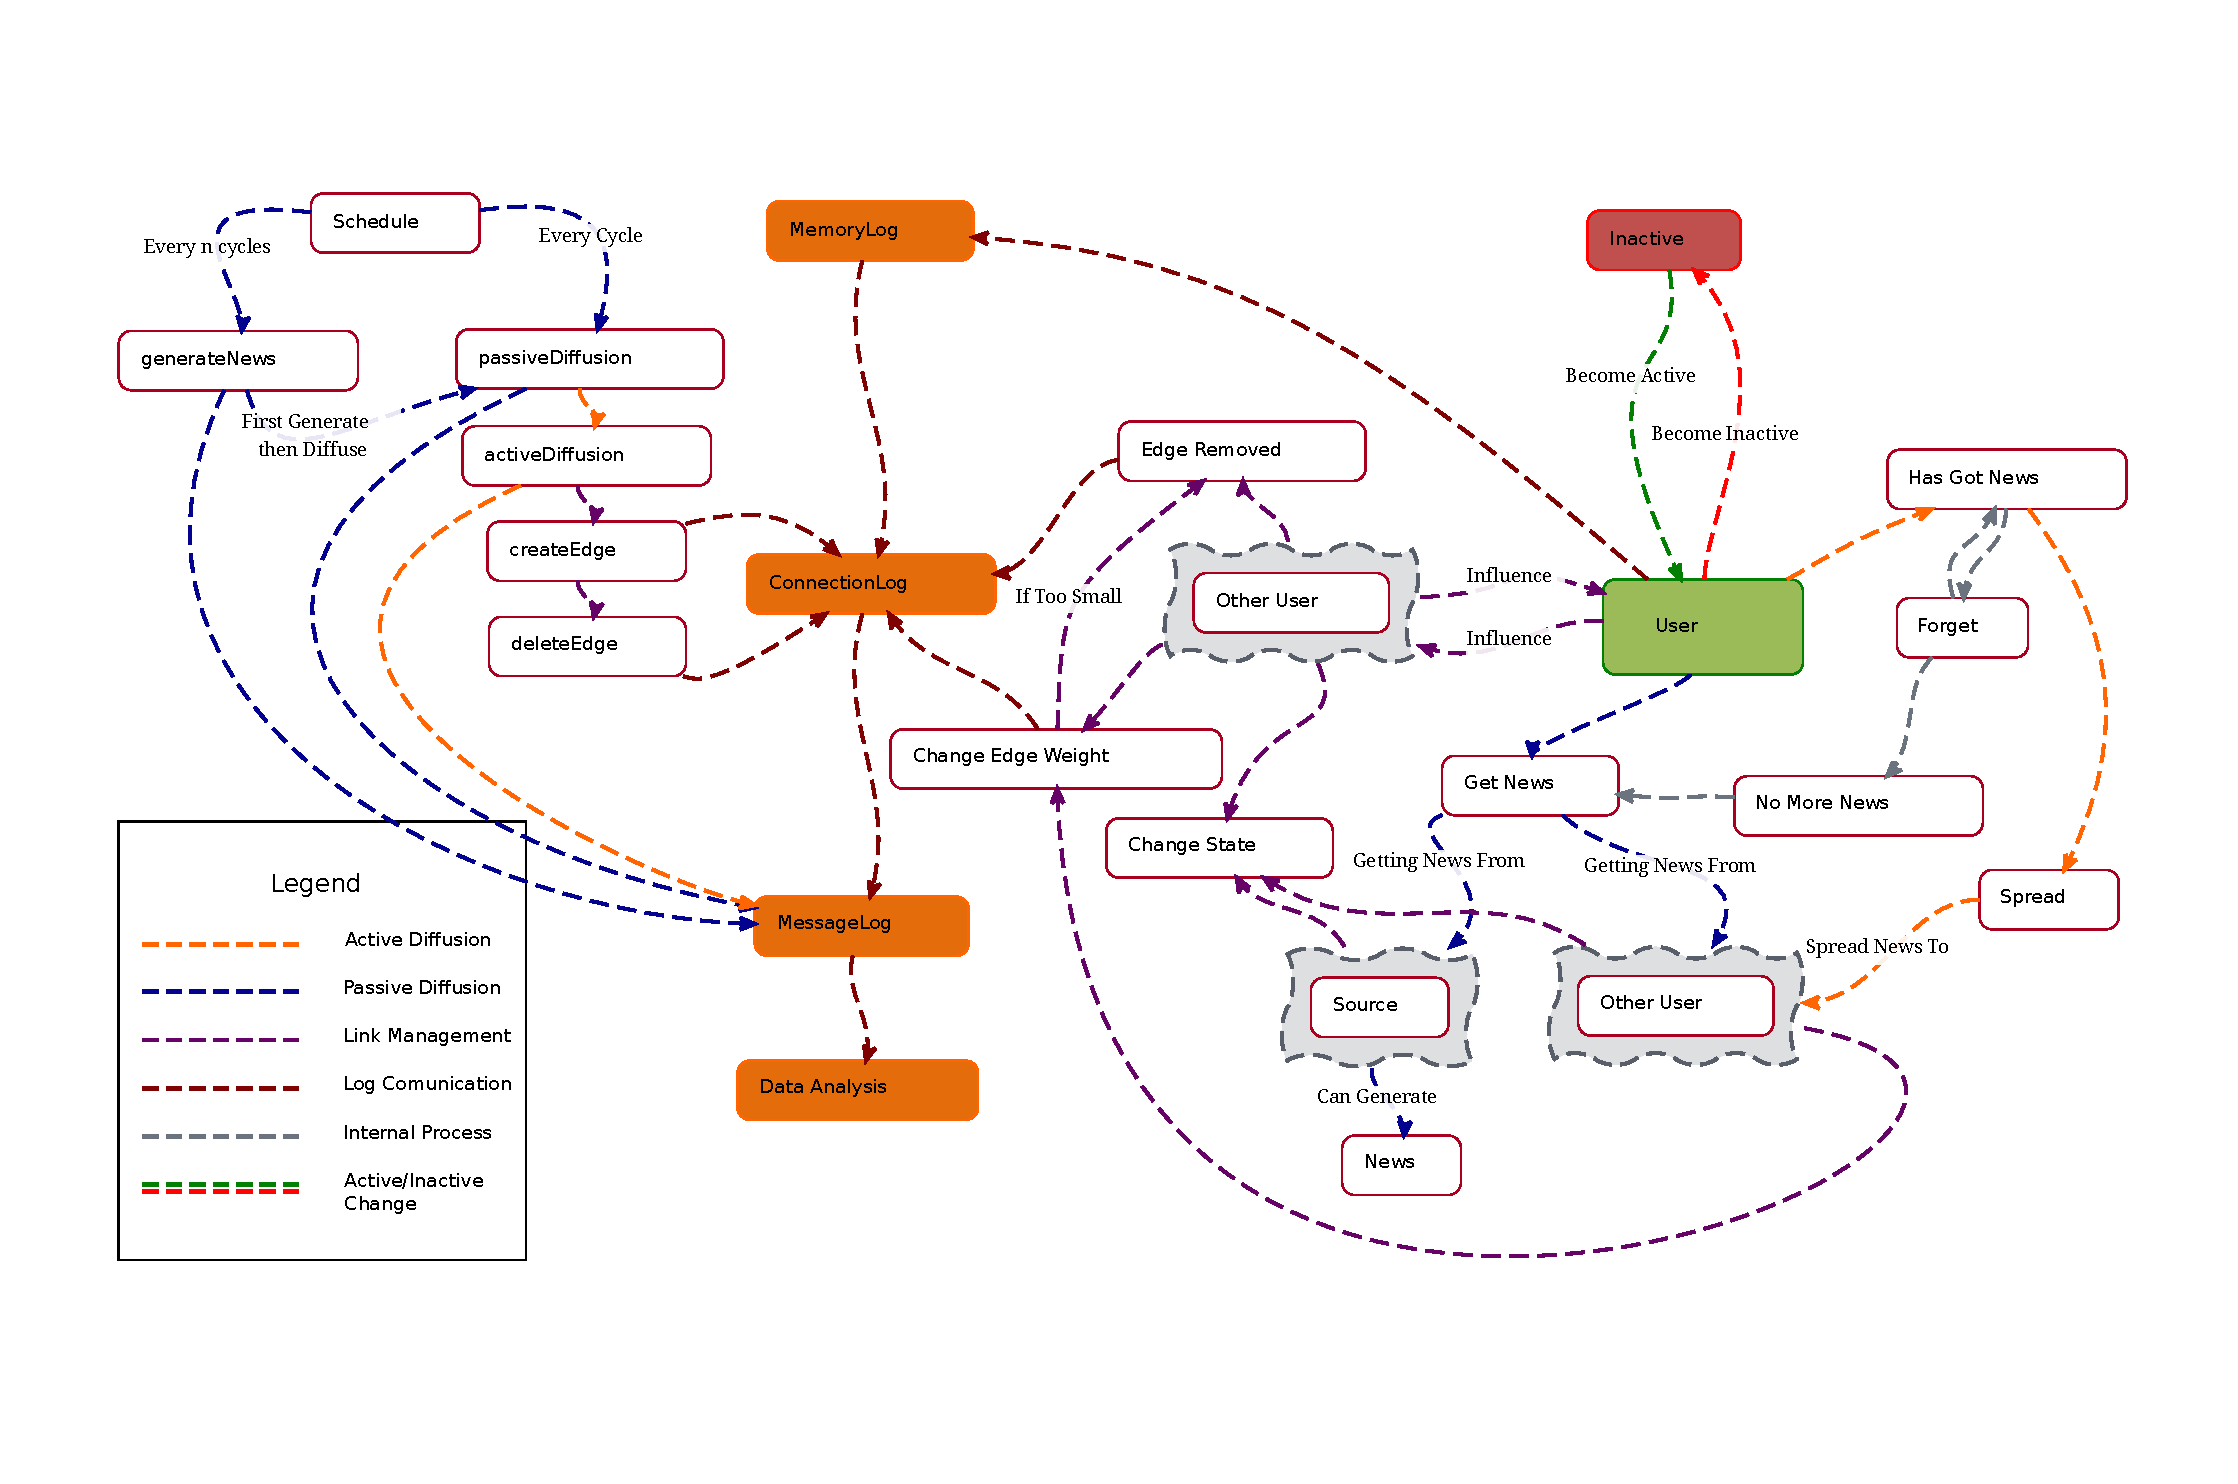
\includegraphics[width=\columnwidth]{mindMap.pdf}
  \label{fig:mindmap}
  \caption{Mind map of the model}
\end{figure}

The agents involved are structured in a hierarchy. 
Schedule: modo per programmare le varie azioni, in ordine temporale esplicitamente dato d noi.  Le azioni possono essere performate con una certa probabilità... removelinks...
Si interfaccia alle azioni generich sopramenzionate.
\\
Le varie Funzioni base (1.2.3.4.5....  9che concatenate costituiscono le azioni vere e proprie degli agenti: Funzioni e metodi delle classi::: SPECCHIETTO
User/Sources
La dinamica del sistema sarà determinata dalle azioni degli utenti; i parametri sopra descritti
influenzeranno le loro decisioni.
\begin{itemize}
\item Agent.py   (user/source) 
\item SkyAgent  (Message scheduler and ConnectionManager ) write the log files...
\item Graph (Create the Graph/ edges and display the graph)
\item Souces
\item Users

\item msglog
\end{itemize}

\section{Tutorial}\label{sec:tutorial}
\subsection{Before the simulation: what to do}\label{subsec:before}
Let us see in practice what we have previously learnt in a simple tutorial:
first of all, we need the whole program, available at \url{https://github.com/BFSteam/memory.}\\
Once downloaded it is convenient to put \texttt{path\_to/memory/src} inside
\texttt{path\_to\_SLAPP3/project.txt} as described in \textit{SLAPP\_Reference\_Handbook.pdf pag20}.
Inside SLAPP3 we can run the program \texttt{runShell.py} from terminal
or from jupyter notebook using \texttt{iRunShell.ipynb}.
The program asks which project we want to run: if we set up the path correctly
we can confirm \textit{memory} path and project.
Afterwards we have to set all the necessary input variables to start
the simulation:
\begin{itemize}
\item[\texttt{Random number seed:}] insert the seed to make the simulation reproducible.
\item[\texttt{Number of sources:}]insert the number of sources inside the network.
\item[\texttt{Number of users:}]insert the number of users inside the network.
\item[\texttt{Average degree for users:}]insert the value of the average degree for users only.
\item[\texttt{Number of cycles:}]insert the maximum number time can reach.
\end{itemize}

In order to simplify our first approach, default values are provided:
answering enter at each line will make the program run, and that's it!\\

\subsection{During the simulation: where to put the accent}\label{subsec:during}
Simulation is running and our network is evolving. A window will appear
with the drawing network\footnote{Graphs drawn using
  \href{https://networkx.github.io/}{networkx} and
  \href{https://matplotlib.org/}{matplotlib}}
and flowing time is displayed in terminal. \\
Nodes of the network are painted with different colors: if they don't
spread, gray for inactive state and blue for active one; if they spread can be orange, pink or cyan depending on the spreaded news.
In detail, every source initially generates a single news, tracked by its color. The source's size are bigger than users and labeled with 0,1 and 2; numbering goes on with users.\\
We show network dynamic in the pictures below:
\begin{figure}[!h]
  \centering
  \begin{subfigure}[t]{.45\textwidth}
    \centering
    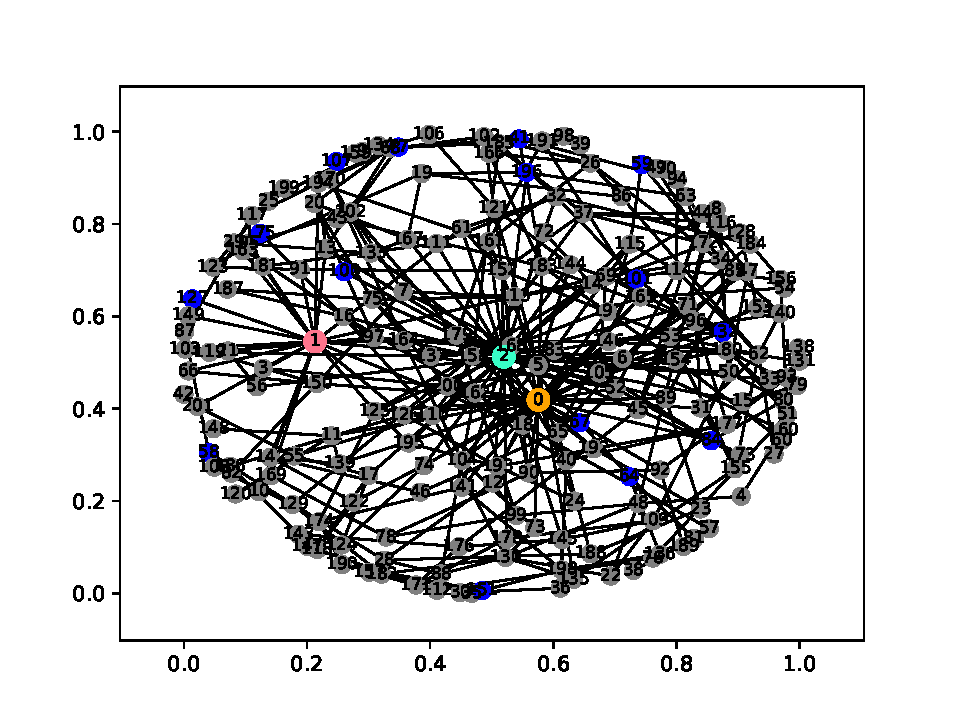
\includegraphics[trim={1cm .5cm 1cm 1cm}, clip, width=\linewidth]{img/pdf/plot-0001.pdf} 
    \caption{1 cycle}
    \label{fig:1}
  \end{subfigure}
  \begin{subfigure}[t]{.45\textwidth}
    \centering
    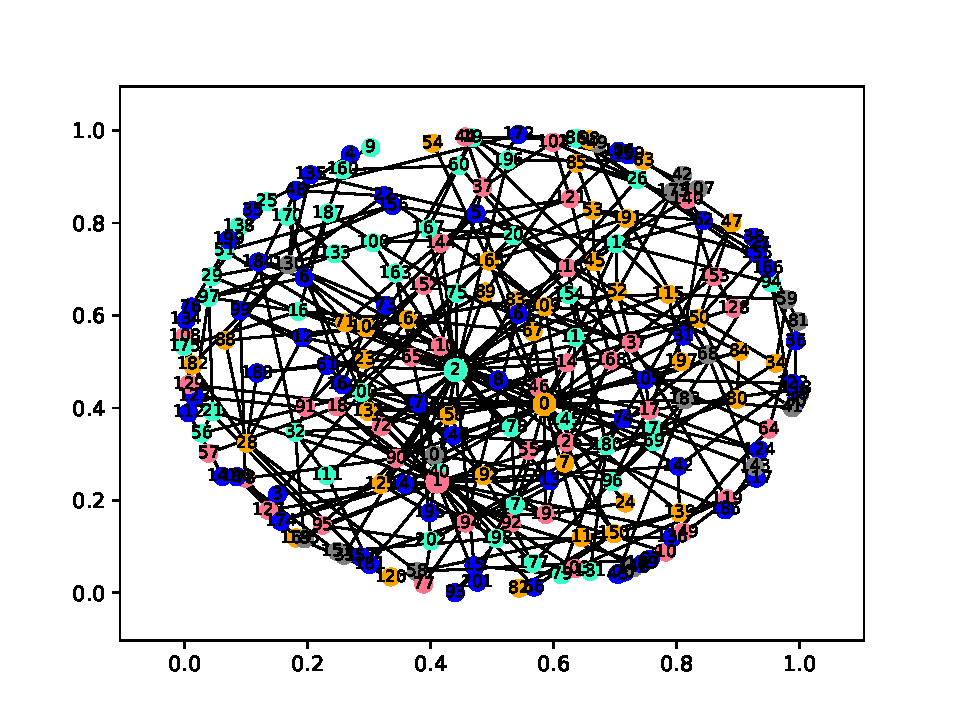
\includegraphics[trim={1cm .5cm 1cm 1cm}, clip, width=\linewidth]{img/pdf/plot-0005.pdf} 
    \caption{5 cycles}
    \label{fig:5}
  \end{subfigure}

  \vspace{0cm}

  \begin{subfigure}[t]{.45\textwidth}
    \centering
    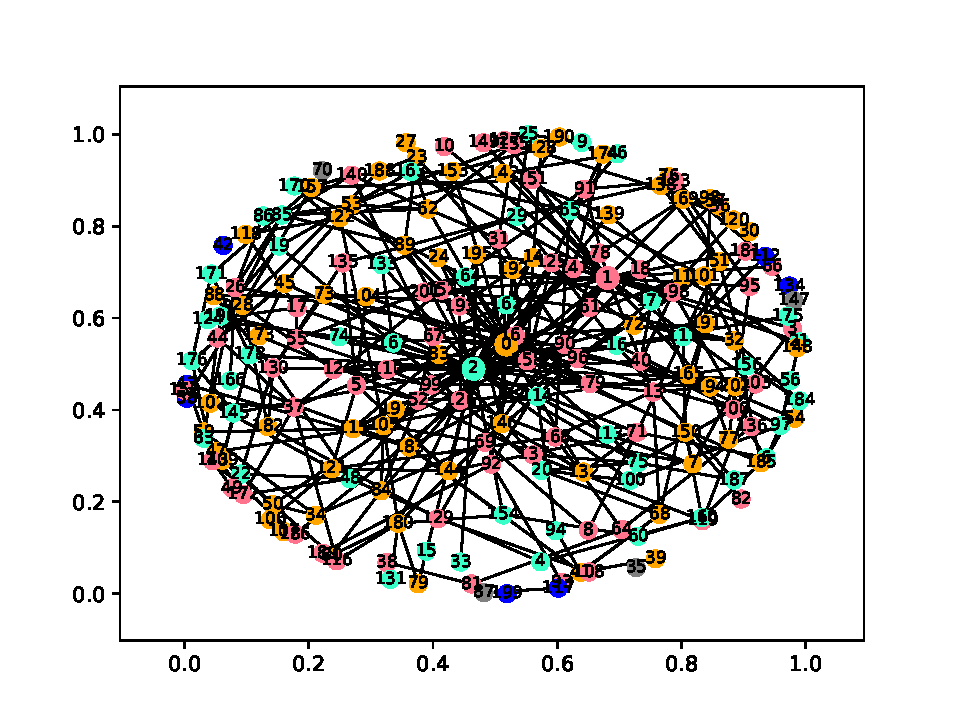
\includegraphics[trim={1cm .5cm 1cm 1cm}, clip, width=\linewidth]{img/pdf/plot-0010.pdf} 
    \caption{10 cycles}
    \label{fig:10}
  \end{subfigure}
  \begin{subfigure}[t]{.45\textwidth}
    \centering
    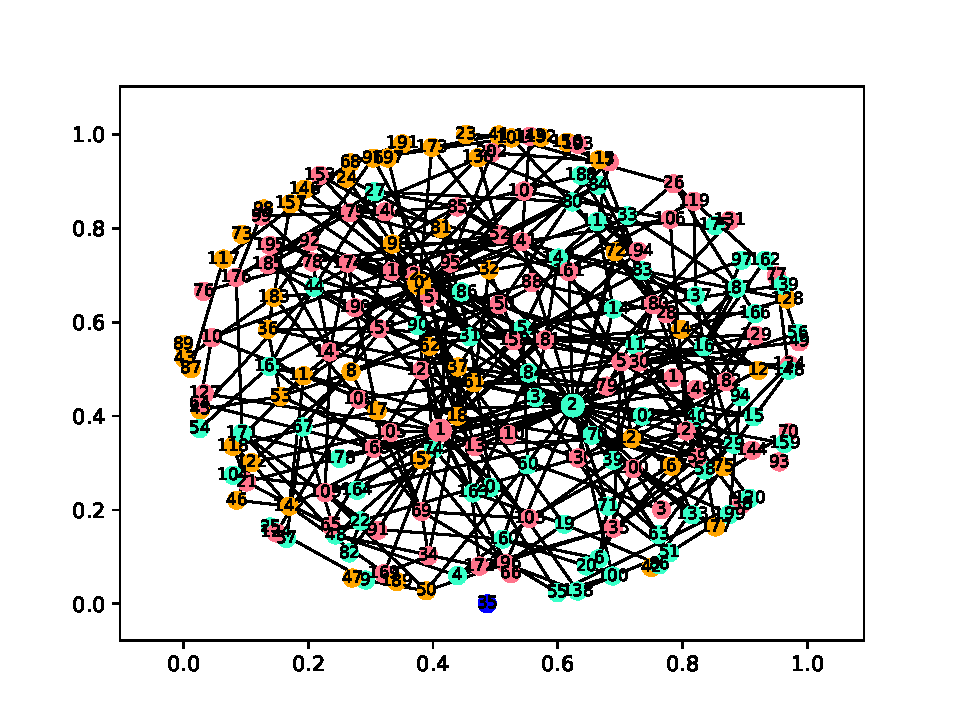
\includegraphics[trim={1cm .5cm 1cm 1cm}, clip, width=\linewidth]{img/pdf/plot-0050.pdf} 
    \caption{50 cycles}
    \label{fig:50}
  \end{subfigure}
 
  \caption{Plot at different initial time steps for a simulation with 3 sources, 200 users, initial average degree of users 3 and 500 time steps. Random seed initialized to 17.}
\end{figure}

\begin{figure}
  \centering
  \begin{subfigure}[t]{.45\textwidth}
    \centering
    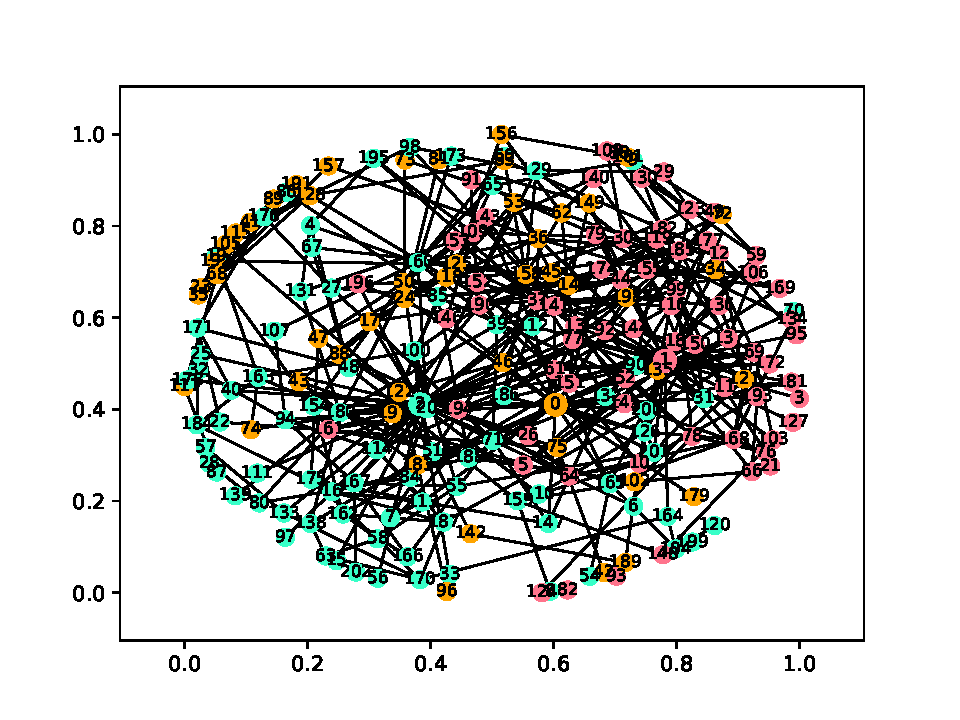
\includegraphics[trim={1cm .5cm 1cm 1cm}, clip, width=\linewidth]{img/pdf/plot-0100.pdf} 
    \caption{100 cycles}
    \label{fig:100}
  \end{subfigure}
  \begin{subfigure}[t]{.45\textwidth}
    \centering
    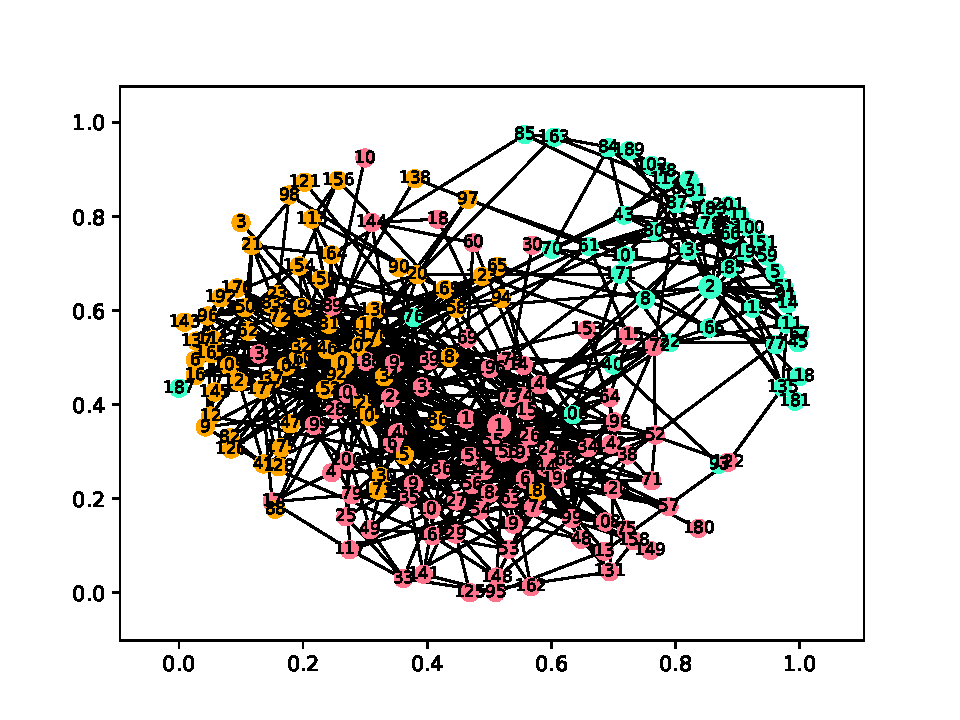
\includegraphics[trim={1cm .5cm 1cm 1cm}, clip, width=\linewidth]{img/pdf/plot-0200.pdf} 
    \caption{200 cycles}
    \label{fig:200}
  \end{subfigure}

  \vspace{0cm}

  \begin{subfigure}[t]{.45\textwidth}
    \centering
    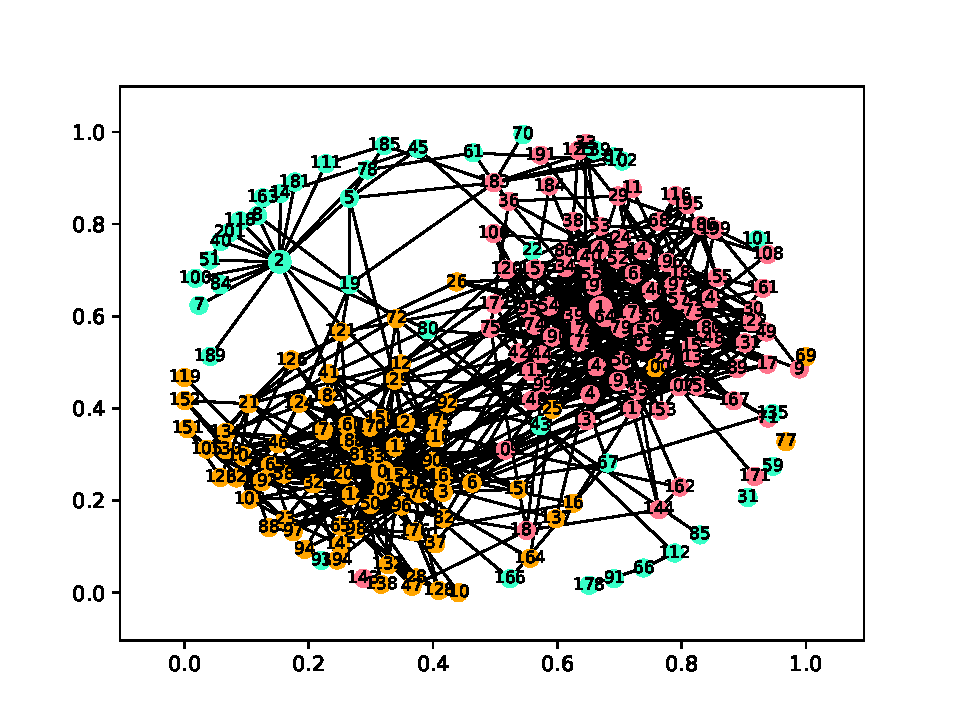
\includegraphics[trim={1cm .5cm 1cm 1cm}, clip, width=\linewidth]{img/pdf/plot-0400.pdf} 
    \caption{400 cycles}
    \label{fig:400}
  \end{subfigure}
  \begin{subfigure}[t]{.45\textwidth}
    \centering
    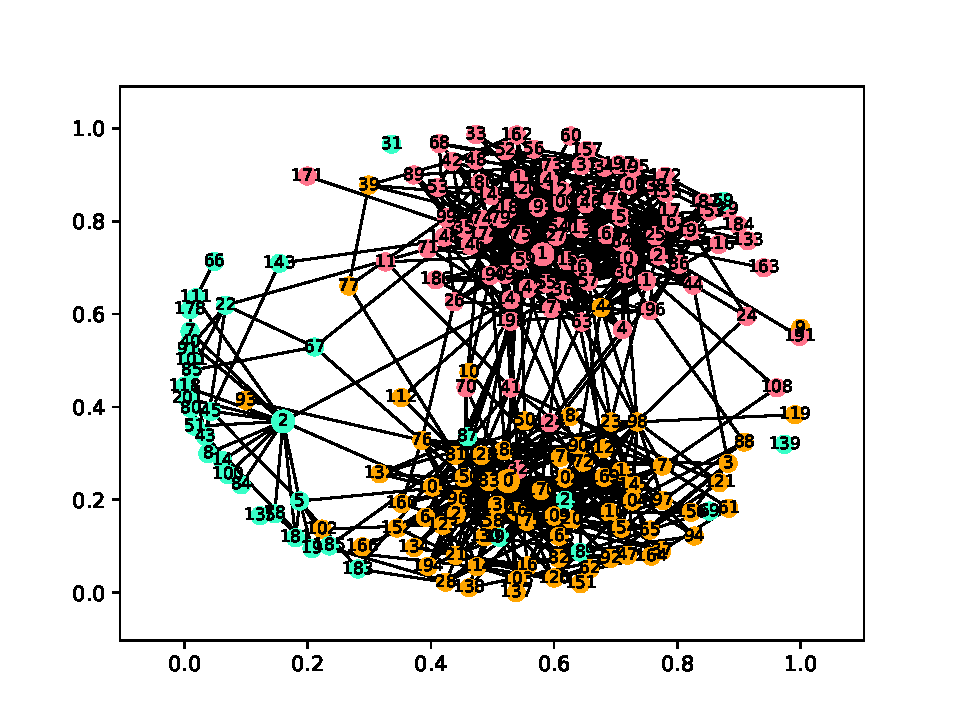
\includegraphics[trim={1cm .5cm 1cm 1cm}, clip, width=\linewidth]{img/pdf/plot-0500.pdf} 
    \caption{500 cycles}
    \label{fig:500}
  \end{subfigure}
 
  \caption{Plot at different final time steps for a simulation with 3 sources, 200 users, initial average degree of users 3 and 500 time steps. Random seed initialized to 17.}
\end{figure}

\subsection{After the simulation: what to notice}\label{subsec:after}
We show graphs of a previous run: the parameters used are, seed 17, 3 sources,
200 users, initial average degree of 3, and 500 time steps.
In figure~\ref{fig:1} we see the net during initialization. Diffusion
has not started yet and users are mostly inactive:
sources have create one news and the few active users are unaware.
After five time steps, figure~\ref{fig:5}, some users have changed their state
to active and started to spread. However, a few of blue users uninformed still remain.
At thenth iteration, in figure~\ref{fig:10}, almost every user
has a news inside and the whole network might a well be homogeneously mixed. 
We have also the first edge creation and remotion, 
consequntly the network's topology start to changing.
Now we jump to the fiftieth iteration, figure~\ref{fig:50},to see that
all the users except one are involved in the dynamic. There is still no
clue of segregation.
After another fifty steps we detect the first clear symptom of segregation.
Moving on of a hundred in a hundred time steps, we see how the orange news
is inclined to disappear and arise a strong segregation in two communities
 due to past influence between users.

\subsection{Further implementations}\label{subsec:implementations}
Some possible future developments are:
\begin{itemize}
\item [adding and removing nodes during execution] can yield big changes
  in the process;
  \item [different algorithm of net generation] at initial clock could be implemented e.g. Barabasi-Albert algorithm or Watts-strogatz algorithm;
\item [look for emerging network behaviors] as said in \textit{\nameref{sec:introduction}} we hope to point out scale-free regime;
\item [analyze the activation time] starting from microscopic behaviors
  it is possible to reproduce macroscopic phenomena such as bursty
  patterns\cite{goh_burstiness_2008}.
\end{itemize}

\subsection{Conclusion}\label{subsec:conclusion}

We would like to emphasize that our model of spreading of news is not based on some epidemic model
 e.g. SIR or another version governed by differential equations. The model instead can be to see like an 
 intersection between a theshold method and a cascade model, founded on microscopic actions made available to agents 
  and based on the common sense and the social realities, for example the RICH PHENOMENON .. mancanza smetto quas


La particolarità del modello puo' essere svelata da semplici osservazioni: più notizie possono diffondersi nella rete e coesistere nella
 dinamica di diffusione; le notizie sono generate da sources che sono parte integrante della rete; si modellizza una memoria individuale
 di ogni agente che gli consente di ricordare un certo numero di news diffuse; si modellizza l'influenza sociale che modifica lo stato mentale;

 \\
 We expect that memory length will lead to measurable macroscopic
 dynamical effects: this is what we would like to investigate.
 This project will advance our understanding on this hypotesis:
 several simulations, performed with different parameters, could lead
 us to a proof which decides the conjecture.
 We observed segregation in almost all examples and some parameters may be
 more important than the others. Two problems arise: what are the key ones
 and if we found them out what their values or their limits would be.
 This is pure speculation on our part but if it were right we could
 establish what parameters are crucial.
 A second issue which we have previously discussed is the question of the
 emerging scale free dynamic: the authenticity of our guess will
 be established through statistical observations.
 


\end{document}

